\chapter{PGP / Gnu Privacy Guard}
Pretty Good Privacy (PGP) pada awalnya adalah aplikasi yang dapat digunakan
pengguna untuk menggunakan kriptografi di berbagai aplikasi dengan lebih mudah.
Pengembangan selanjutnya PGP menjadi bagian dari {\em public key
infrastructure}.

\section{Sejarah}
[... more to be written ...]

Gnu Privacy Guard (GPG) merupakan implementasi dari PGP yang bersifat terbuka.
(Catatan: Singkatan dari GPG ini merupakan guyonan terhadap PGP.) Bab ini akan
membahas lebih banyak tentang GGP, meskipun konsep yang sama dapat juga
diterapkan pada PGP jika Anda menggunakan produk PGP yang komersial.

Dalam buku ini, kita akan menggunakan GPG versi {\em command line interface},
yaitu dengan mengetikkan perintah ``gpg'' di program terminal atau CMD.exe.
Ada banyak program {\em GUI} dari GPG ini. Silahkan gunakan manual terkait
dengan program-program tersebut. Prinsipnya masih tetap sama.

\section{Menggunakan Gnu Privacy Guard, gpg}
Awal dari penggunakan GPG adalah membuat pasangan kunci publik dan privat. Hal
ini dapat dilakukan dengan menggunakan perintah berikut.

\begin{verbatim}
gpg --key-gen
\end{verbatim}

Perintah di atas akan menanyakan beberapa hal, seperti jenis algoritma yang
digunakan (pilih RSA dan RSA), panjang kuncinya (pilih 2048), dan alamat email
yang akan digunakan untuk kunci tersebut. Dalam contoh buku ini saya akan
menggunakan alamat email ``rahard2017@gmail.com''. Gunakan alamat email Anda
sebagai penggantinya/

\begin{verbatim}
$ gpg --gen-key
gpg (GnuPG/MacGPG2) 2.0.30; Copyright (C) 2015 Free Software Foundation, Inc.
This is free software: you are free to change and redistribute it.
There is NO WARRANTY, to the extent permitted by law.

Please select what kind of key you want:
   (1) RSA and RSA (default)
   (2) DSA and Elgamal
   (3) DSA (sign only)
   (4) RSA (sign only)
Your selection? 1
RSA keys may be between 1024 and 4096 bits long.
What keysize do you want? (2048)
Requested keysize is 2048 bits
Please specify how long the key should be valid.
         0 = key does not expire
      <n>  = key expires in n days
      <n>w = key expires in n weeks
      <n>m = key expires in n months
      <n>y = key expires in n years
      Key is valid for? (0) 3m
Key expires at Wed May 31 10:30:37 2017 WIB
Is this correct? (y/N) y

GnuPG needs to construct a user ID to identify your key.

Real name: Budi Rahardjo
Email address: rahard2017b@gmail.com
Comment:
You selected this USER-ID:
    "Budi Rahardjo <rahard2017@gmail.com>"

Change (N)ame, (C)omment, (E)mail or (O)kay/(Q)uit?
\end{verbatim}

Setelah proses {\em key generation} selesai, kunci publik dapat diekspor dengan
menggunakan perintah  berikut. Gantikan ``rahard2017@gmail.com'' dengan alamat
email Anda.

\begin{verbatim}
gpg --export --armor rahard2017@gmail.com > kunci-public.asc
\end{verbatim}

Akan dihasilkan berkas ``kunci-public.asc''. Tanpa perintah {\em redirect
output} yang menggunakan ``>'' itu, hasilnya hanya akan ditampilkan di layar
saja. Tentu saja Anda dapat menggunakan nama berkas lainnya.
Berikut ini adalah contoh beberapa baris pertama dari berkas ASCII hasil ekspor
kunci tersebut. (Tampilan bisa panjang sekali, bergantung dari panjang kunci
yang digunakan.)

\begin{verbatim}
-----BEGIN PGP PUBLIC KEY BLOCK-----
Comment: GPGTools - https://gpgtools.org

mQENBFiiijUBCAD3ZIxjUQyDtcGTmHs2iU+2aS+MMp2w+codVRrqLfVI+V8S+TmP
WGe2Gu4pTLovGzZ2NGWvKACZ0A+BL97e9K6QN6+UIYRArFdxfojQ4lbwH/WO1YSn
J6BsCE1IfX8niRiskdibBhZZcrUCcDa/tgvgXTymoAeZEcMwR48hEOUWuOGoCE2g
TA/kD9yCyorFUKEsbyKJMKPtlMJGICUwtggDdXT5arCCafpydLGxok+w4TJjADeX
jeTxDgYSNjCNar9wRhtnG+G/Irbfctj77/9Ppz8j8Dp1NkAwx5P+9AJRNNkwU88c
7FSEz0cpAzgC4VyaL/iX85G8wr6z5kaWNV3FABEBAAG0JEJ1ZGkgUmFoYXJkam8g
PHJhaGFyZDIwMTdAZ21haWwuY29tPokBPQQTAQoAJwUCWKKKNQIbAwUJABuvgAUL
...
\end{verbatim}

Kunci publik ini yang akan didistribusikan secara publik, misal disimpan di
blog Anda. Kunci ini juga dapat disimpan di {\em key server}.

Untuk melihat informasi mengenai kunci Anda, dapat digunakan perintah berikut:

\begin{verbatim}
gpg --fingerprint rahard2017

pub   2048R/EB6CEB46 2017-02-14 [expires: 2017-03-07]
      Key fingerprint = 810B 2149 3366 E699 F95E  9E49 07E1 BDC5 EB6C EB46
uid       [ultimate] Budi Rahardjo <rahard2017@gmail.com>
sub   2048R/C2E83C60 2017-02-14 [expires: 2017-03-07]
\end{verbatim}

Perhatikan bahwa kunci publik yang ini memiliki ID ``EB6CEB46''. ID ini dapat
digunakan untuk bertukar kunci, atau untuk melakukan proses-proses lainnya.
Sebagai contoh, kita dapat mengirimkan kunci ini ke server agar dapat dilihat
atau dicari oleh orang lain. Keyserver yang akan kita gunakan dalam contoh ini
adalah pgp.mit.edu.

\begin{verbatim}
gpg --keyserver pgp.mit.edu --send-keys EB6CEB46
\end{verbatim}

Pengirimkan kunci dapat juga dilakukan dengan menggunakan web dari situs PGP
MIT tersebut sebagaimana dicontohkan dalam gambar berikut.

\begin{figure}[ht]
\fbox{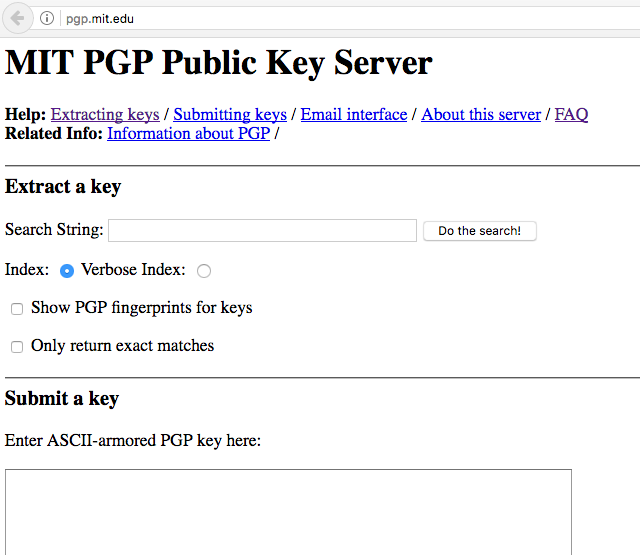
\includegraphics[width=1.0\linewidth]{graphics/pgp-mit.png}}
\caption{Key server pgp.mit.edu}
\label{fig:pgp-mit}
\end{figure}


\section{Tools}
Perintah-perintah dalam contoh pada bagian sebelumnya dilakukan dengan
menggunakan {\em command line}. Ada beberapa {\em tools} yang dapat membantu
untuk mempermudah operasi.


\subsection{Web of Trust}
Keamanan dari PGP/GPG ini berbasis {\em web of trust}. Bagaimana kita dapat
mempercayai bahwa kunci publik tersebut milik dari ``Budi Rahardjo'' dengan
alamat email tersebut (rahard2017@gmail.com)? Boleh jadi ada seseorang yang
dengan sengaja memalsukan identitas tersebut. 

Proses verifikasi dilakukan oleh orang lain dengan menandatangani kunci
tersebut dan kemudian data tersebut - kunci yang sudah ditandatagani - diunggah
kembali ke keyserver. 
